%%%%%%%%%%%%%%%%%%%%%%%%%%%%%%%%%%%%%%%%%
% Beamer Presentation
% LaTeX Template
% Version 1.0 (10/11/12)
%
% This template has been downloaded from:
% http://www.LaTeXTemplates.com
%
% License:
% CC BY-NC-SA 3.0 (http://creativecommons.org/licenses/by-nc-sa/3.0/)
%
%%%%%%%%%%%%%%%%%%%%%%%%%%%%%%%%%%%%%%%%%

%----------------------------------------------------------------------------------------
%	PACKAGES AND THEMES
%----------------------------------------------------------------------------------------

\documentclass{beamer}

\mode<presentation> {

% The Beamer class comes with a number of default slide themes
% which change the colors and layouts of slides. Below this is a list
% of all the themes, uncomment each in turn to see what they look like.

%\usetheme{default}
%\usetheme{AnnArbor}
%\usetheme{Antibes}
%\usetheme{Bergen}
%\usetheme{Berkeley}
%\usetheme{Berlin}
%\usetheme{Boadilla}
%\usetheme{CambridgeUS}
%\usetheme{Copenhagen}
%\usetheme{Darmstadt}
%\usetheme{Dresden}
%\usetheme{Frankfurt}
%\usetheme{Goettingen}
%\usetheme{Hannover}
%\usetheme{Ilmenau}
%\usetheme{JuanLesPins}
%\usetheme{Luebeck}
\usetheme{Madrid}
%\usetheme{Malmoe}
%\usetheme{Marburg}
%\usetheme{Montpellier}
%\usetheme{PaloAlto}
%\usetheme{Pittsburgh}
%\usetheme{Rochester}
%\usetheme{Singapore}
%\usetheme{Szeged}
%\usetheme{Warsaw}

% As well as themes, the Beamer class has a number of color themes
% for any slide theme. Uncomment each of these in turn to see how it
% changes the colors of your current slide theme.

%\usecolortheme{albatross}
%\usecolortheme{beaver}
%\usecolortheme{beetle}
%\usecolortheme{crane}
%\usecolortheme{dolphin}
%\usecolortheme{dove}
%\usecolortheme{fly}
%\usecolortheme{lily}
%\usecolortheme{orchid}
%\usecolortheme{rose}
%\usecolortheme{seagull}
%\usecolortheme{seahorse}
%\usecolortheme{whale}
%\usecolortheme{wolverine}

%\setbeamertemplate{footline} % To remove the footer line in all slides uncomment this line
%\setbeamertemplate{footline}[page number] % To replace the footer line in all slides with a simple slide count uncomment this line

%\setbeamertemplate{navigation symbols}{} % To remove the navigation symbols from the bottom of all slides uncomment this line
}

\usepackage{graphicx} % Allows including images
\usepackage{booktabs} % Allows the use of \toprule, \midrule and \bottomrule in tables

%----------------------------------------------------------------------------------------
%	TITLE PAGE
%----------------------------------------------------------------------------------------

\title[LODES]{LODES (Library of ODE Solvers)} % The short title appears at the bottom of every slide, the full title is only on the title page

\author{Paul Aoanan} % Your name
\institute[McMaster University] % Your institution as it will appear on the bottom of every slide, may be shorthand to save space
{
CAS 741\\
McMaster University \\ % Your institution for the title page
\medskip
%\textit{john@smith.com} % Your email address
}
\date{\today} % Date, can be changed to a custom date

\begin{document}

\begin{frame}
\titlepage % Print the title page as the first slide
\end{frame}

\begin{frame}
\frametitle{Overview} % Table of contents slide, comment this block out to remove it
\tableofcontents % Throughout your presentation, if you choose to use \section{} and \subsection{} commands, these will automatically be printed on this slide as an overview of your presentation
\end{frame}

%----------------------------------------------------------------------------------------
%	PRESENTATION SLIDES
%----------------------------------------------------------------------------------------

%------------------------------------------------
\section{Module Hierarchy} % Sections can be created in order to organize your presentation into discrete blocks, all sections and subsections are automatically printed in the table of contents as an overview of the talk
%------------------------------------------------

%\subsection{Subsection Example} % A subsection can be created just before a set of slides with a common theme to further break down your presentation into chunks

\begin{frame}
\frametitle{Module Hierarchy}

\begin{figure}[H]
\centering
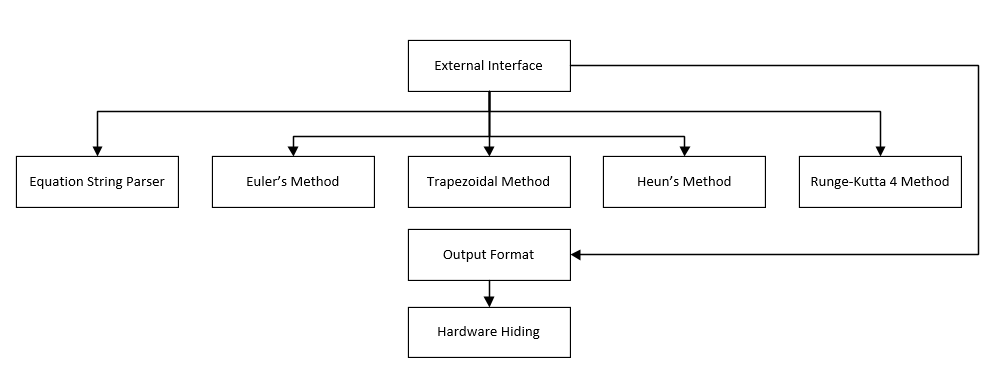
\includegraphics[width=0.9\textwidth]{use.png}
\caption{Use Hierarchy Among Modules}
\label{FigUH}
\end{figure}

\end{frame}

%------------------------------------------------

\section{Modules for Discussion}

%------------------------------------------------


\subsection {External Interface}

\begin{frame}
\frametitle{External Interface}
\begin{itemize}
\item Uses:
	\begin{itemize}
		\item Equation Parser, Euler's Method, Trapezoidal Method, Heun's Method, Runge-Kutta 4 Method, Output
	\end{itemize}
\item Syntax:
	\begin{itemize}
		\item Access Routine Semantics:
			\begin{itemize}
			\item parseEquation()\\
				Input: User-input ODE string\\
				Output: Machine-interpreted ODE\\
			\item euler()\\
				Input: Machine-interpreted ODE, x\_0, y\_0, x\_k, h
				Output: y\_k, success
			\item trap()\\
				Input: Machine-interpreted ODE, x\_0, y\_0, x\_k, h
				Output: y\_k, success
			\item heun()\\
				Input: Machine-interpreted ODE, x\_0, y\_0, x\_k, h
				Output: y\_k, success
			\item rk()\\
				Input: Machine-interpreted ODE, x\_0, y\_0, x\_k, h
				Output: y\_k, success
			\item output()\\
				Input: y\_k, success
				Output: Screen Display
			\end{itemize}
		\item Exceptions:
			\begin{itemize}
			\item badEq, badX0, badY0, badXK, badH, error				
			\end{itemize}
	\end{itemize}
\end{itemize}
\end{frame}

%------------------------------------------------

\subsection {Euler's Method}

\begin{frame}
\frametitle{Euler's Method}
\begin{itemize}
\item Uses:
	\begin{itemize}
		\item none
	\end{itemize}
\item Syntax:
	\begin{itemize}
		\item Input: Machine-interpreted ODE (f), x\_0, y\_0, x\_k, h
		\item Output: y\_k, success
	\end{itemize}
\end{itemize}
\end{frame}

\begin{frame}
\frametitle{Euler's Method}
\begin{itemize}
\item Semantics:
	\begin{itemize}
		\item output: y\_k, success\\
		\begin{itemize}
		\item Pseudo-code:\\
			success = false;
			x(1) = x\_0;\\
			y(1) = y\_0;\\
			N =  (x\_0 - x\_k) / h\\
			for n = 1 to N \\% For loop, sets next t,y values
				x(n+1) = x(n) + h;\\
				y(n+1)=y(n) + h * f(x(n), y(n));\\
			end\\
			y\_k = y(N)\\
			success = true\\
			return y\_k, success
		\end{itemize}
	\end{itemize}
\end{itemize}
\end{frame}

%------------------------------------------------


\subsection {Heun's Method}

\begin{frame}
\frametitle{Heun's Method}
\begin{itemize}
\item Uses:
	\begin{itemize}
		\item none
	\end{itemize}
\item Syntax:
	\begin{itemize}
		\item Input: Machine-interpreted ODE (f), x\_0, y\_0, x\_k, h
		\item Output: y\_k, success
	\end{itemize}
\end{itemize}
\end{frame}

\begin{frame}
\frametitle{Heun's Method}
\begin{itemize}
\item Semantics:
	\begin{itemize}
		\item output: y\_k, success\\
		\begin{itemize}
		\item Pseudo-code:\\
			success = false;
			x(1) = x\_0;\\
			y(1) = y\_0;\\
			N =  (x\_0 - x\_k) / h\\
			for n = 1 to N \\% For loop, sets next t,y values
				x(n+1) = x(n) + h;\\
				y(n+1)=y(n) + (h/2) * [f(x(n), y(n)) + f(x(n) + h, y(n) + h * f(x(n), y(n)))];\\
			end\\
			y\_k = y(N)\\
			success = true\\
			return y\_k, success
		\end{itemize}
	\end{itemize}
\end{itemize}
\end{frame}


%------------------------------------------------


\subsection {Output Format}

\begin{frame}
\frametitle{Output Format}
\begin{itemize}
\item Uses:
	\begin{itemize}
		\item Hardware Hiding
	\end{itemize}
\item Syntax:
	\begin{itemize}
		\item Input: y\_k, success
		\item Output: y\_k, success
	\end{itemize}
\end{itemize}
\end{frame}


\begin{frame}
\Huge{\centerline{The End}}
\end{frame}

%----------------------------------------------------------------------------------------

\end{document} 